% ============================================================
% ANLP Assignment 1 - Report skeleton (structure only, no analysis).
% You write every sentence of prose yourself, per the assignment's
% "do not use AI to write your final report" rule.
%
% Formatting matches the spec: 12pt, Times New Roman, 1-inch margins,
% max 6 pages excluding references/links.
%
% This file is OUTSIDE rollnumber_assignment1/ on purpose - compile it,
% fill it in, export Report.pdf, and drop that into the submission
% folder yourself. Delete this .tex from the submission zip.
%
% Compile: pdflatex Report_template.tex (or use Overleaf / VS Code LaTeX Workshop)
% ============================================================
\documentclass[12pt]{article}
\usepackage[margin=1in]{geometry}
\usepackage{times}
\usepackage{booktabs}
\usepackage{graphicx}
\usepackage{subcaption}
\usepackage{hyperref}
\usepackage{amsmath}

\title{Assignment 1: Transformers from Scratch, Architectural Variants,\\ and Byte Latent Transformers (BLT)}
\author{Your Name \\ Roll Number}
\date{\today}

\begin{document}
\maketitle

% ------------------------------------------------------------
\section{Overview}
% Guiding questions to answer in 4-6 sentences:
% - What is the task (binary-cipher -> plaintext seq2seq)?
% - What does the dataset look like (5,000 pairs, Brown corpus sentences,
%   letters+space only, exact 8-bits-per-char cipher)?
% - What are you studying (5 controlled ablations: pos. encoding, attention,
%   normalization, tokenization)?
[Write 4-6 sentences here.]

% ------------------------------------------------------------
\section{Architecture (Task 1)}

\subsection{Base Transformer}
% Describe your encoder-decoder skeleton: embedding -> (+PE) -> N encoder
% layers -> N decoder layers -> output projection. Mention pre-norm residual
% placement and why you chose it (stability at your depth/LR).
[Write 3-5 sentences here.]

\subsection{Attention: MHA vs.\ GQA}
% Briefly state the scaled dot-product attention formula (already given in
% the assignment PDF) and how GQA differs (n_kv_heads shared via
% repeat_interleave). State the n_heads / n_kv_heads you used and why.
[Write 3-5 sentences here.]

\subsection{Positional Encoding: Sinusoidal vs.\ RoPE}
% State where each is applied (sinusoidal: added once to embeddings;
% RoPE: applied inside self-attention on Q/K only, not cross-attention -
% explain briefly why not cross-attention).
[Write 3-5 sentences here.]

\subsection{Normalization: LayerNorm vs.\ RMSNorm}
% One or two sentences on the mechanical difference (RMSNorm drops the
% mean-centering / bias term) and why it's cheaper.
[Write 2-3 sentences here.]

\subsection{Byte Latent Transformer (C5)}
% Describe your simplified BLT: fixed-size byte patches -> LocalEncoder
% (byte embed + small transformer + attention pooling) -> global transformer
% (same base architecture as C1) -> LocalDecoder (autoregressive byte
% prediction per patch, conditioned on the patch's global context vector).
% State your patch_size and why you picked it.
[Write 5-7 sentences here.]

% ------------------------------------------------------------
\section{Experimental Setup}

% TODO: fill in the actual values you trained with (must be identical
% across C1-C5 except for the one changed axis).
\begin{table}[h]
\centering
\caption{Shared hyperparameters across all five configurations.}
\begin{tabular}{ll}
\toprule
Hyperparameter & Value \\
\midrule
$d_{model}$ & [ ] \\
Attention heads & [ ] \\
KV heads (GQA only) & [ ] \\
Encoder/decoder layers & [ ] \\
FFN dimension & [ ] \\
Dropout & [ ] \\
BLT patch size & [ ] \\
Max sequence length (chars) & [ ] \\
Subword vocab size & [ ] \\
Batch size & [ ] \\
Learning rate (peak) & [ ] \\
LR schedule & [ ] \\
Epochs & [ ] \\
Train / val / test split & 80\% / 10\% / 10\% \\
Optimizer & AdamW \\
Hardware & [ ] \\
\bottomrule
\end{tabular}
\end{table}

% Mention decoding strategy (greedy, per the spec) and anything notable
% about the dataset property you exploited (source-byte-count ==
% target-char-count) if relevant to your setup.
[Write 2-4 sentences here.]

% ------------------------------------------------------------
\section{Results}

% Pull these numbers straight from outputs/results.json after all 5 configs
% finish training.
\begin{table}[h]
\centering
\caption{Test-set metrics across configurations. BLEU/ROUGE only apply to
tokenized (subword) models.}
\small
\begin{tabular}{lcccccc}
\toprule
Config & Bit-Acc (\%) & Seq-Acc (\%) & Levenshtein & BLEU & ROUGE-L & Peak GPU (MB) \\
\midrule
C1 (base)        & [ ] & [ ] & [ ] & [ ] & [ ] & [ ] \\
C2 (RoPE)        & [ ] & [ ] & [ ] & [ ] & [ ] & [ ] \\
C3 (GQA)         & [ ] & [ ] & [ ] & [ ] & [ ] & [ ] \\
C4 (RMSNorm)     & [ ] & [ ] & [ ] & [ ] & [ ] & [ ] \\
C5 (BLT)         & [ ] & [ ] & [ ] & --  & --  & [ ] \\
\bottomrule
\end{tabular}
\end{table}

% Also worth a row/column, from outputs/results.json "params" and your
% WandB run durations: parameter count and wall-clock time/epoch per config
% (especially C1 vs C5, since the assignment explicitly asks about training
% speed/overhead).

\begin{figure}[h]
\centering
% Use the bar charts run_all.sh already generates in outputs/plots/
\begin{subfigure}{0.48\textwidth}
  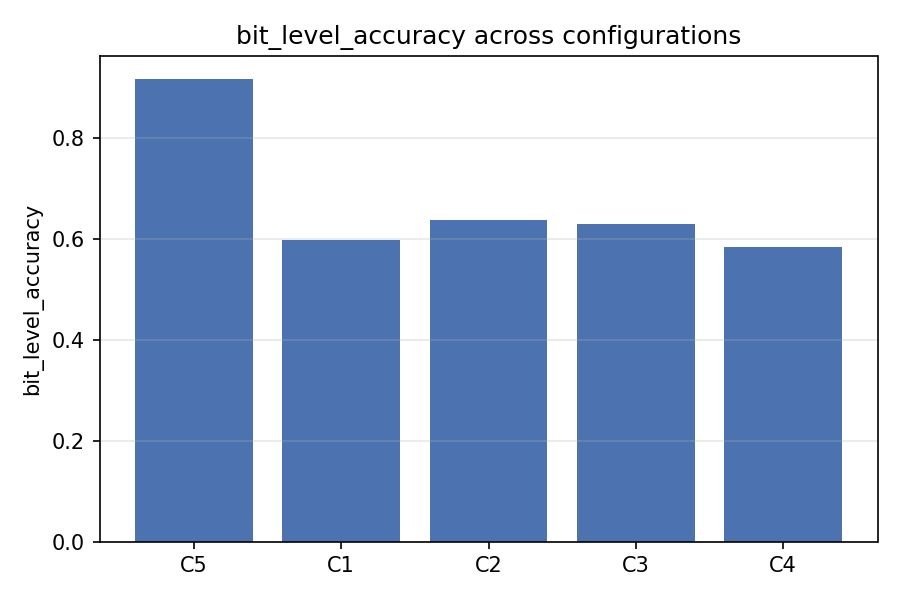
\includegraphics[width=\linewidth]{outputs/plots/compare_bit_level_accuracy.png}
  \caption{Bit-level accuracy}
\end{subfigure}
\hfill
\begin{subfigure}{0.48\textwidth}
  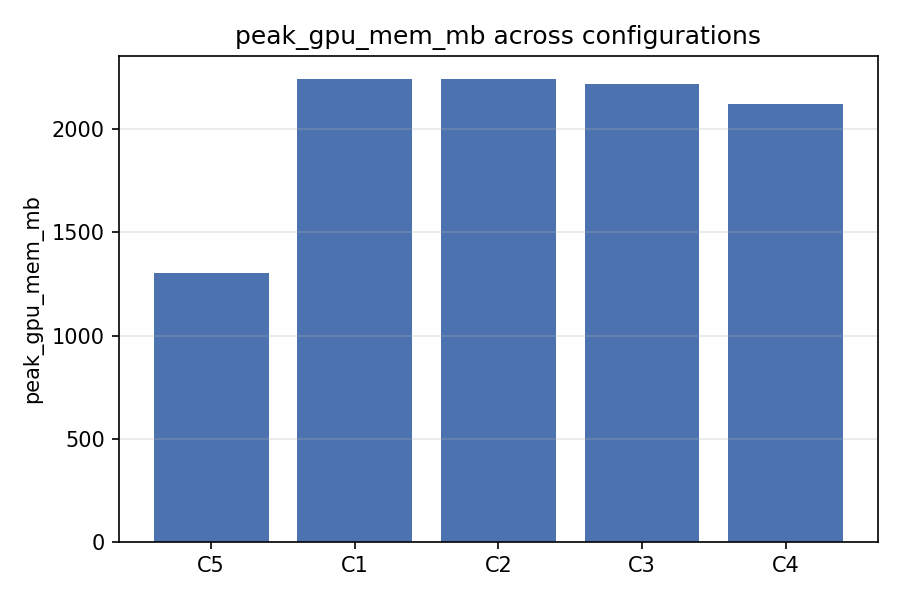
\includegraphics[width=\linewidth]{outputs/plots/compare_peak_gpu_mem_mb.png}
  \caption{Peak GPU memory}
\end{subfigure}
\caption{Cross-configuration comparison.}
\end{figure}

% Optional: a compact grid of the 5 per-config loss curves
% (outputs/plots/<CFG>/loss_curve.png) using subcaption, if space allows.

% ------------------------------------------------------------
\section{Ablation Analysis}
% This section is the core of the "analysis" grade. For each config, name
% the specific mechanism and connect it to what the numbers actually show.
% Don't just restate the table - explain *why* you think the effect happened.

\subsection{C2 vs.\ C1: RoPE vs.\ Sinusoidal Absolute}
% Did RoPE help or hurt? Faster/slower convergence (check loss curves)?
% Any hypothesis tied to sequence length or the cipher's structure?
[Write 3-5 sentences here.]

\subsection{C3 vs.\ C1: Grouped-Query vs.\ Multi-Head Attention}
% Parameter count difference, any accuracy/speed tradeoff observed,
% whether it matches your expectation given n_kv_heads.
[Write 3-5 sentences here.]

\subsection{C4 vs.\ C1: RMSNorm vs.\ LayerNorm}
% Training stability differences, final metric differences, anything
% about gradient norms from your WandB logs worth mentioning.
[Write 3-5 sentences here.]

\subsection{C5 vs.\ C1: Token-Free BLT vs.\ Subword Tokenization}
% This is the subsection the assignment explicitly calls out - cover:
% - Training speed / step time
% - Peak GPU memory usage
% - Sequence reconstruction quality (bit-level and sequence accuracy,
%   since BLEU/ROUGE don't apply here)
% - Your own take on the memory-vs-accuracy tradeoff, tied to *why* BLT's
%   two-level (patch + byte) architecture costs what it costs.
[Write 5-8 sentences here.]

% ------------------------------------------------------------
\section{Conclusion}
% 3-5 sentences: which single change helped most/least, and one honest
% limitation of your setup (e.g. max_chars truncation, dataset size,
% epoch budget) that you'd address with more compute/time.
[Write 3-5 sentences here.]

% ------------------------------------------------------------
% Not counted toward the 6-page limit per the assignment instructions.
\clearpage
\section*{Links}
\begin{itemize}
  \item WandB project: \url{[paste link]}
  \item Hugging Face checkpoints: \url{[paste link]}
\end{itemize}

\end{document}
